\documentclass{article}

\usepackage{amsmath, amssymb}
\usepackage{physics}
\usepackage{french}
\usepackage[margin=2.5cm]{geometry}
\usepackage{graphicx}

\begin{document}

\title{Devoir 4 : Simulation Monte Carlo du modèle de Ising}
\author{PHQ404}
\date{Remise : 14 avril 2022 à 23h59}
\maketitle

\section{Objectif}

L'objectif de ce devoir est d'étudier une transition de phase
dans le modèle de Ising en 2 dimensions.

\section{Comment présenter et remettre votre TP}

Vous devez créer un dépôt Git pour votre devoir.
Dans ce dépôt, on doit retrouver le code permettant de réaliser le devoir 
ainsi qu'un court rapport. 
Le nom de votre dépot doit être \textit{devoir4\_personne1\_personne2}.
Pour le code, vous devez utiliser Poetry pour gérer votre environnement virtuel.

De plus, le fichier README de votre projet doit indiquer comment obtenir le rapport.
Celui-ci peut-être effectué en \LaTeX\ ou à l'aide d'un carnet numérique (Jupyter ou autre).
Si vous utilisez un carnet, celui-ci ne doit contenir que le code nécessaire pour votre rapport.
Les implémentations doivent se trouver dans un module que vous importez.
Si vous utilisez \LaTeX, il n'est pas nécessaire de soumettre le rapport compilé.
Il est suffisant d'indiquer quel fichier compiler pour obtenir le rapport.

Sauf indication contraire de votre part, 
la dernière version de votre dépôt avant la remise sera évaluée.

\section{Énoncé}

\subsection{Modèle de Ising}

Un fichier python est joint à ce devoir. 
Celui-ci contient une classe nommée \textit{Ising} qui permet de représenter 
un système de spins ferromagnétique avec un couplage entre les premiers voisins.
La classe est cependant incomplète et vous devez compléter l'implémentation 
de certaines méthodes. 
Pour ce faire, vous pouvez ajouter des méthodes intermédiaires, 
mais vous ne pouvez pas retirer de méthodes.

La classe est compilée avec la bibliothèque \textit{NumBa} pour accélérer les calculs.
Cependant, cela impose des contraintes sur les versions de \textit{NumPy}.
En effet, il est important de choisir une version de numpy avant 1.22 pour éviter des problèmes 
de compatibilité.

\subsection{Méthode du binning}

Une seconde classe nommée \textit{Observable} est également fournise pour 
évaluer des statistiques sur l'aimantation et l'énergie à l'aide de la méthode du binning.
Vous devez également compléter cette classe.

\subsection{Simulation Monte Carlo}

À l'aide de ces deux classes, vous devez implémenter une simulation Monte Carlo 
pour un système de $32 \times 32$ spins pour des températures entre $1.0$ et $4.0$ 
par incrément de $0.1$.
Pour ce faire, vous devez
\begin{enumerate}
    \item initialiser le système aléatoirement;
    \item effectuer 1 000 000 d'itérations pour réchauffer le système;
    \item rendre une mesure de l'énergie et de l'aimantation après chaque interval de 1 000 itérations;
    \item terminer la simulation après avoir accumuler $2^{16}$ mesures;
    \item enregistrer les résultats dans un fichier de données.
\end{enumerate}

\subsection{Visualisation des résultats}

Vous devez fournir des graphiques similaires aux figures suivantes 
et commenter brièvement les résultats.

\begin{figure}[h]
    \begin{center}
        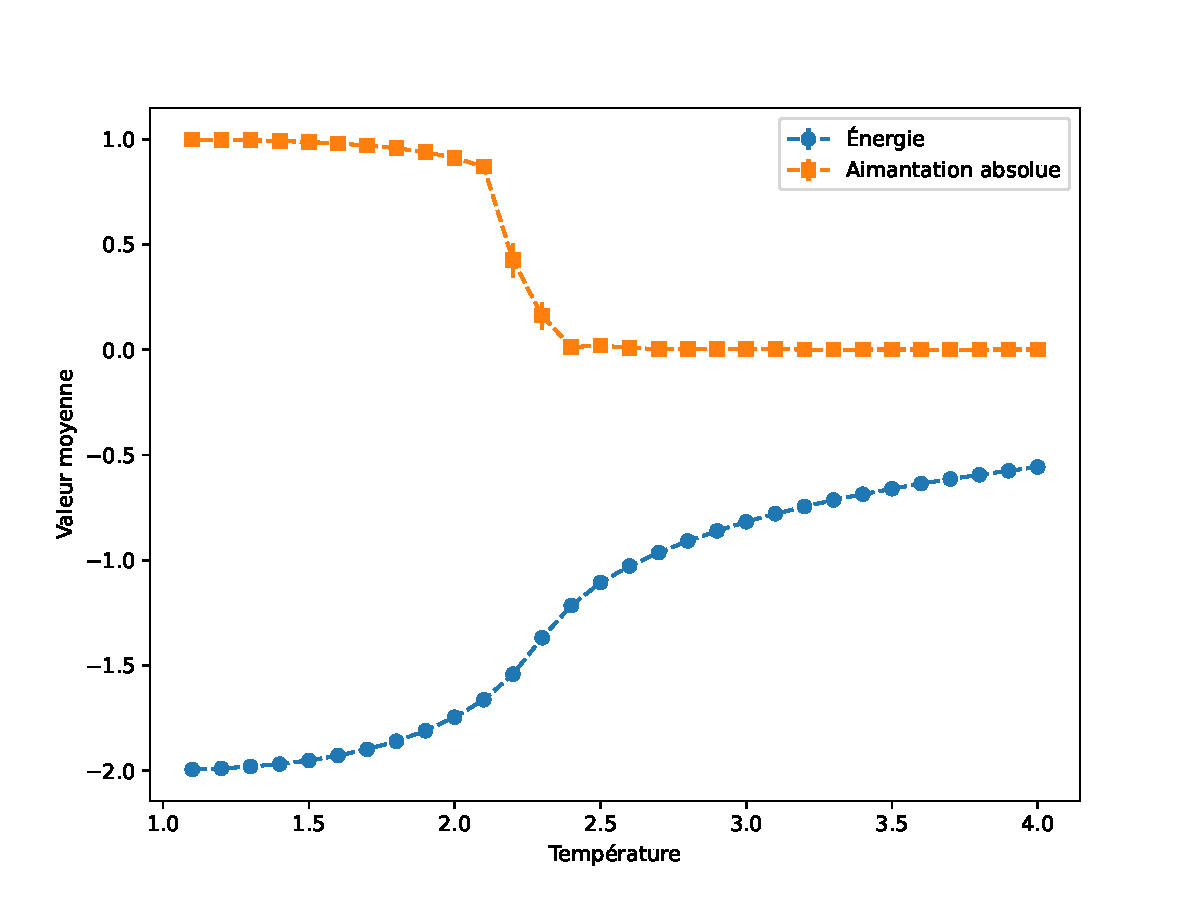
\includegraphics[width=0.45\textwidth]{./energie_aimantation.pdf}
    \end{center}
    \caption{
        Exemple de figure pour les valeurs moyennes et les erreurs d'estimation
        pour l'énergie et l'aimantation par spin selon la température.
        Les erreurs d'estimation sont obtenues avec la méthode du binning de 16 niveaux.
    }
    \label{fig:moyennes}
\end{figure}

\begin{figure}[h]
    \begin{center}
        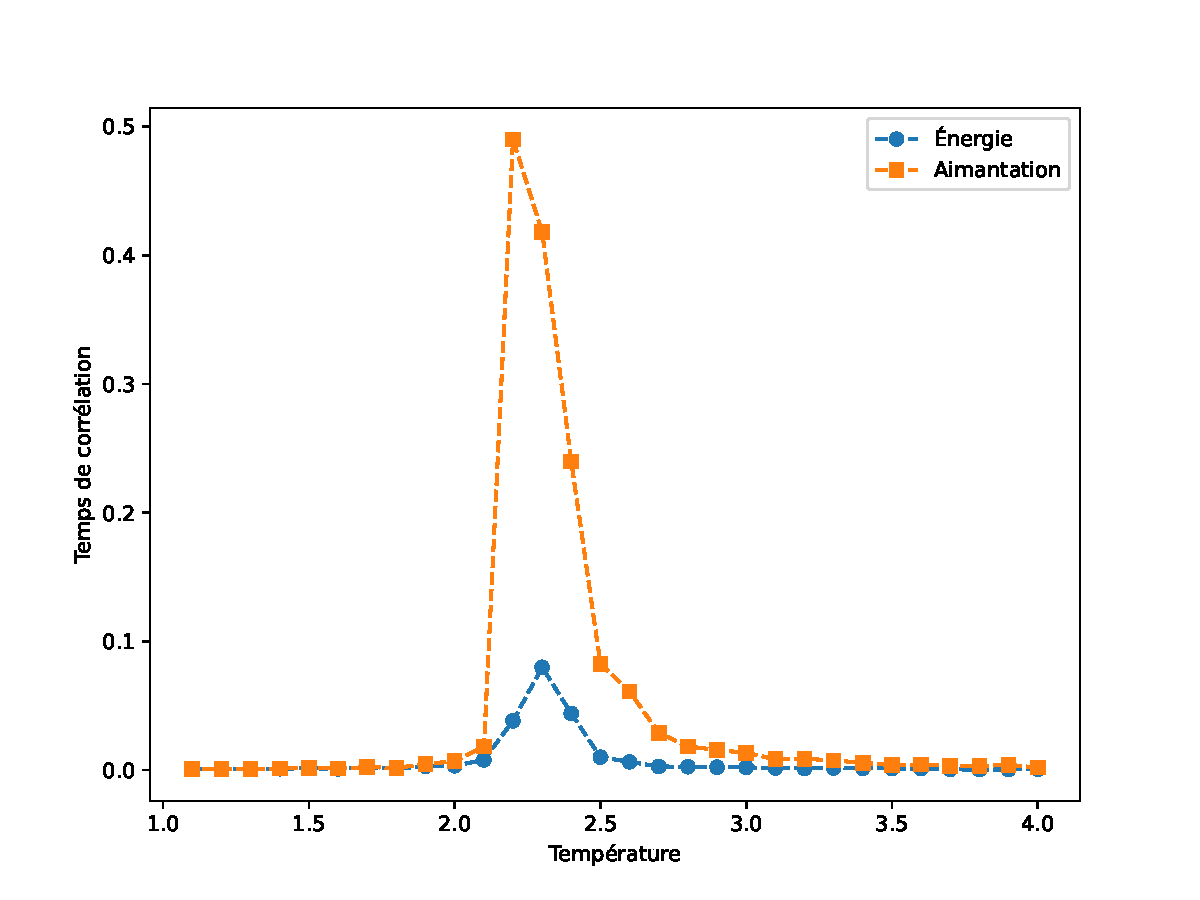
\includegraphics[width=0.45\textwidth]{./temps_correlation.pdf}
    \end{center}
    \caption{
        Exemple de figure pour les temps de corrélation selon la température.
    }
    \label{fig:correlation}
\end{figure}


\section{Critères d'évaluation}

\begin{description}
    \item[30 points] Pour compléter la classe \textit{Ising}.
    \item[30 points] Pour compléter la classe \textit{Observable}.
    \item[30 points] Pour l'implémentation de la simulation Monte Carlo.
    \item[10 points] Pour la qualité générale du rapport et des graphiques.
\end{description}

\end{document}
